% Options for packages loaded elsewhere
\PassOptionsToPackage{unicode}{hyperref}
\PassOptionsToPackage{hyphens}{url}
%
\documentclass[
]{article}
\usepackage{amsmath,amssymb}
\usepackage{iftex}
\ifPDFTeX
  \usepackage[T1]{fontenc}
  \usepackage[utf8]{inputenc}
  \usepackage{textcomp} % provide euro and other symbols
\else % if luatex or xetex
  \usepackage{unicode-math} % this also loads fontspec
  \defaultfontfeatures{Scale=MatchLowercase}
  \defaultfontfeatures[\rmfamily]{Ligatures=TeX,Scale=1}
\fi
\usepackage{lmodern}
\ifPDFTeX\else
  % xetex/luatex font selection
\fi
% Use upquote if available, for straight quotes in verbatim environments
\IfFileExists{upquote.sty}{\usepackage{upquote}}{}
\IfFileExists{microtype.sty}{% use microtype if available
  \usepackage[]{microtype}
  \UseMicrotypeSet[protrusion]{basicmath} % disable protrusion for tt fonts
}{}
\makeatletter
\@ifundefined{KOMAClassName}{% if non-KOMA class
  \IfFileExists{parskip.sty}{%
    \usepackage{parskip}
  }{% else
    \setlength{\parindent}{0pt}
    \setlength{\parskip}{6pt plus 2pt minus 1pt}}
}{% if KOMA class
  \KOMAoptions{parskip=half}}
\makeatother
\usepackage{xcolor}
\usepackage[margin=1in]{geometry}
\usepackage{color}
\usepackage{fancyvrb}
\newcommand{\VerbBar}{|}
\newcommand{\VERB}{\Verb[commandchars=\\\{\}]}
\DefineVerbatimEnvironment{Highlighting}{Verbatim}{commandchars=\\\{\}}
% Add ',fontsize=\small' for more characters per line
\usepackage{framed}
\definecolor{shadecolor}{RGB}{248,248,248}
\newenvironment{Shaded}{\begin{snugshade}}{\end{snugshade}}
\newcommand{\AlertTok}[1]{\textcolor[rgb]{0.94,0.16,0.16}{#1}}
\newcommand{\AnnotationTok}[1]{\textcolor[rgb]{0.56,0.35,0.01}{\textbf{\textit{#1}}}}
\newcommand{\AttributeTok}[1]{\textcolor[rgb]{0.13,0.29,0.53}{#1}}
\newcommand{\BaseNTok}[1]{\textcolor[rgb]{0.00,0.00,0.81}{#1}}
\newcommand{\BuiltInTok}[1]{#1}
\newcommand{\CharTok}[1]{\textcolor[rgb]{0.31,0.60,0.02}{#1}}
\newcommand{\CommentTok}[1]{\textcolor[rgb]{0.56,0.35,0.01}{\textit{#1}}}
\newcommand{\CommentVarTok}[1]{\textcolor[rgb]{0.56,0.35,0.01}{\textbf{\textit{#1}}}}
\newcommand{\ConstantTok}[1]{\textcolor[rgb]{0.56,0.35,0.01}{#1}}
\newcommand{\ControlFlowTok}[1]{\textcolor[rgb]{0.13,0.29,0.53}{\textbf{#1}}}
\newcommand{\DataTypeTok}[1]{\textcolor[rgb]{0.13,0.29,0.53}{#1}}
\newcommand{\DecValTok}[1]{\textcolor[rgb]{0.00,0.00,0.81}{#1}}
\newcommand{\DocumentationTok}[1]{\textcolor[rgb]{0.56,0.35,0.01}{\textbf{\textit{#1}}}}
\newcommand{\ErrorTok}[1]{\textcolor[rgb]{0.64,0.00,0.00}{\textbf{#1}}}
\newcommand{\ExtensionTok}[1]{#1}
\newcommand{\FloatTok}[1]{\textcolor[rgb]{0.00,0.00,0.81}{#1}}
\newcommand{\FunctionTok}[1]{\textcolor[rgb]{0.13,0.29,0.53}{\textbf{#1}}}
\newcommand{\ImportTok}[1]{#1}
\newcommand{\InformationTok}[1]{\textcolor[rgb]{0.56,0.35,0.01}{\textbf{\textit{#1}}}}
\newcommand{\KeywordTok}[1]{\textcolor[rgb]{0.13,0.29,0.53}{\textbf{#1}}}
\newcommand{\NormalTok}[1]{#1}
\newcommand{\OperatorTok}[1]{\textcolor[rgb]{0.81,0.36,0.00}{\textbf{#1}}}
\newcommand{\OtherTok}[1]{\textcolor[rgb]{0.56,0.35,0.01}{#1}}
\newcommand{\PreprocessorTok}[1]{\textcolor[rgb]{0.56,0.35,0.01}{\textit{#1}}}
\newcommand{\RegionMarkerTok}[1]{#1}
\newcommand{\SpecialCharTok}[1]{\textcolor[rgb]{0.81,0.36,0.00}{\textbf{#1}}}
\newcommand{\SpecialStringTok}[1]{\textcolor[rgb]{0.31,0.60,0.02}{#1}}
\newcommand{\StringTok}[1]{\textcolor[rgb]{0.31,0.60,0.02}{#1}}
\newcommand{\VariableTok}[1]{\textcolor[rgb]{0.00,0.00,0.00}{#1}}
\newcommand{\VerbatimStringTok}[1]{\textcolor[rgb]{0.31,0.60,0.02}{#1}}
\newcommand{\WarningTok}[1]{\textcolor[rgb]{0.56,0.35,0.01}{\textbf{\textit{#1}}}}
\usepackage{graphicx}
\makeatletter
\def\maxwidth{\ifdim\Gin@nat@width>\linewidth\linewidth\else\Gin@nat@width\fi}
\def\maxheight{\ifdim\Gin@nat@height>\textheight\textheight\else\Gin@nat@height\fi}
\makeatother
% Scale images if necessary, so that they will not overflow the page
% margins by default, and it is still possible to overwrite the defaults
% using explicit options in \includegraphics[width, height, ...]{}
\setkeys{Gin}{width=\maxwidth,height=\maxheight,keepaspectratio}
% Set default figure placement to htbp
\makeatletter
\def\fps@figure{htbp}
\makeatother
\setlength{\emergencystretch}{3em} % prevent overfull lines
\providecommand{\tightlist}{%
  \setlength{\itemsep}{0pt}\setlength{\parskip}{0pt}}
\setcounter{secnumdepth}{-\maxdimen} % remove section numbering
\usepackage{fontspec}
\setmainfont{Times New Roman}
\usepackage{ctex}
\ifLuaTeX
  \usepackage{selnolig}  % disable illegal ligatures
\fi
\usepackage{bookmark}
\IfFileExists{xurl.sty}{\usepackage{xurl}}{} % add URL line breaks if available
\urlstyle{same}
\hypersetup{
  pdftitle={homework4},
  pdfauthor={黄舟翔 3220103606},
  hidelinks,
  pdfcreator={LaTeX via pandoc}}

\title{homework4}
\author{黄舟翔 3220103606}
\date{2025-06-29}

\begin{document}
\maketitle

We continue examining the diffusion of tetracycline among doctors in
Illinois in the early 1950s, building on our work in lab 6. You will
need the data sets \texttt{ckm\_nodes.csv} and \texttt{ckm\_network.dat}
from the labs.

\subsubsection{1.}\label{section}

Clean the data to eliminate doctors for whom we have no adoption-date
information, as in the labs. Only use this cleaned data in the rest of
the assignment.

用以下代码完成:

\begin{Shaded}
\begin{Highlighting}[]
\NormalTok{ckm\_nodes }\OtherTok{\textless{}{-}} \FunctionTok{read\_csv}\NormalTok{(}\StringTok{\textquotesingle{}data/ckm\_nodes.csv\textquotesingle{}}\NormalTok{)}
\NormalTok{noinfor }\OtherTok{\textless{}{-}} \FunctionTok{which}\NormalTok{(}\FunctionTok{is.na}\NormalTok{(ckm\_nodes}\SpecialCharTok{$}\NormalTok{adoption\_date))}
\NormalTok{ckm\_nodes }\OtherTok{\textless{}{-}}\NormalTok{ ckm\_nodes[}\SpecialCharTok{{-}}\NormalTok{noinfor, ]}
\NormalTok{ckm\_network }\OtherTok{\textless{}{-}} \FunctionTok{read.table}\NormalTok{(}\StringTok{\textquotesingle{}data/ckm\_network.dat\textquotesingle{}}\NormalTok{)}
\NormalTok{ckm\_network }\OtherTok{\textless{}{-}}\NormalTok{ ckm\_network[}\SpecialCharTok{{-}}\NormalTok{noinfor, }\SpecialCharTok{{-}}\NormalTok{noinfor]}
\end{Highlighting}
\end{Shaded}

\subsubsection{2.}\label{section-1}

Create a new data frame which records, for every doctor, for every
month, whether that doctor began prescribing tetracycline that month,
whether they had adopted tetracycline before that month, the number of
their contacts who began prescribing strictly \emph{before} that month,
and the number of their contacts who began prescribing in that month or
earlier. Explain why the dataframe should have 6 columns, and 2125 rows.

用以下代码完成:

\begin{Shaded}
\begin{Highlighting}[]
\CommentTok{\# 添加医生 ID 列(使用行号作为唯一标识)}
\NormalTok{ckm\_nodes}\SpecialCharTok{$}\NormalTok{doctor\_id }\OtherTok{\textless{}{-}} \DecValTok{1}\SpecialCharTok{:}\FunctionTok{nrow}\NormalTok{(ckm\_nodes)}
\NormalTok{n\_doctors }\OtherTok{\textless{}{-}} \FunctionTok{nrow}\NormalTok{(ckm\_nodes)}
\NormalTok{adoption\_dates }\OtherTok{\textless{}{-}}\NormalTok{ ckm\_nodes}\SpecialCharTok{$}\NormalTok{adoption\_date}
\CommentTok{\# 创建所有医生{-}月份组合 (125 医生 × 17 个月 = 2125 行)}
\NormalTok{doctor\_months }\OtherTok{\textless{}{-}} \FunctionTok{expand.grid}\NormalTok{(}
\AttributeTok{doctor\_id =}\NormalTok{ ckm\_nodes}\SpecialCharTok{$}\NormalTok{doctor\_id,}
\AttributeTok{month =} \DecValTok{1}\SpecialCharTok{:}\DecValTok{17}\NormalTok{,}
\AttributeTok{stringsAsFactors =} \ConstantTok{FALSE}
\NormalTok{)}
\CommentTok{\# 添加关键指标列}
\NormalTok{doctor\_months}\SpecialCharTok{$}\NormalTok{adopted\_this\_month }\OtherTok{\textless{}{-}} \FunctionTok{with}\NormalTok{(doctor\_months, \{}
\FunctionTok{as.integer}\NormalTok{(adoption\_dates[doctor\_id] }\SpecialCharTok{==}\NormalTok{ month)}
\NormalTok{\})}
\NormalTok{doctor\_months}\SpecialCharTok{$}\NormalTok{already\_adopted }\OtherTok{\textless{}{-}} \FunctionTok{with}\NormalTok{(doctor\_months, \{}
\FunctionTok{as.integer}\NormalTok{(adoption\_dates[doctor\_id] }\SpecialCharTok{\textless{}}\NormalTok{ month)}
\NormalTok{\})}
\CommentTok{\# 预计算每个医生的邻居索引}
\NormalTok{neighbor\_indices }\OtherTok{\textless{}{-}} \FunctionTok{lapply}\NormalTok{(}\DecValTok{1}\SpecialCharTok{:}\NormalTok{n\_doctors, }\ControlFlowTok{function}\NormalTok{(i) \{}
\FunctionTok{which}\NormalTok{(ckm\_network[i, ] }\SpecialCharTok{==} \DecValTok{1}\NormalTok{)}
\NormalTok{\})}
\CommentTok{\# 计算邻居采用指标}
\NormalTok{doctor\_months}\SpecialCharTok{$}\NormalTok{n\_contacts\_adopted\_before }\OtherTok{\textless{}{-}} \FunctionTok{mapply}\NormalTok{(}\ControlFlowTok{function}\NormalTok{(doc\_id, t) \{}
\NormalTok{neighbors }\OtherTok{\textless{}{-}}\NormalTok{ neighbor\_indices[[doc\_id]]}
\ControlFlowTok{if}\NormalTok{(}\FunctionTok{length}\NormalTok{(neighbors) }\SpecialCharTok{\textgreater{}} \DecValTok{0}\NormalTok{) \{}
\FunctionTok{sum}\NormalTok{(adoption\_dates[neighbors] }\SpecialCharTok{\textless{}}\NormalTok{ t, }\AttributeTok{na.rm =} \ConstantTok{TRUE}\NormalTok{)}
\NormalTok{\} }\ControlFlowTok{else}\NormalTok{ \{}
\DecValTok{0}
\NormalTok{\}}
\NormalTok{\}, doctor\_months}\SpecialCharTok{$}\NormalTok{doctor\_id, doctor\_months}\SpecialCharTok{$}\NormalTok{month)}
\NormalTok{doctor\_months}\SpecialCharTok{$}\NormalTok{n\_contacts\_adopted\_by\_now }\OtherTok{\textless{}{-}} \FunctionTok{mapply}\NormalTok{(}\ControlFlowTok{function}\NormalTok{(doc\_id, t) \{}
\NormalTok{neighbors }\OtherTok{\textless{}{-}}\NormalTok{ neighbor\_indices[[doc\_id]]}
\ControlFlowTok{if}\NormalTok{(}\FunctionTok{length}\NormalTok{(neighbors) }\SpecialCharTok{\textgreater{}} \DecValTok{0}\NormalTok{) \{}
\FunctionTok{sum}\NormalTok{(adoption\_dates[neighbors] }\SpecialCharTok{\textless{}=}\NormalTok{ t, }\AttributeTok{na.rm =} \ConstantTok{TRUE}\NormalTok{)}
\NormalTok{\} }\ControlFlowTok{else}\NormalTok{ \{}
\DecValTok{0}
\NormalTok{\}}
\NormalTok{\}, doctor\_months}\SpecialCharTok{$}\NormalTok{doctor\_id, doctor\_months}\SpecialCharTok{$}\NormalTok{month)}
\CommentTok{\# 验证结果}
\FunctionTok{cat}\NormalTok{(}\StringTok{" 行数:"}\NormalTok{, }\FunctionTok{nrow}\NormalTok{(doctor\_months), }\StringTok{" 预期: 125 医生 × 17 个月 = 2125}\SpecialCharTok{\textbackslash{}n}\StringTok{"}\NormalTok{)}
\end{Highlighting}
\end{Shaded}

\begin{verbatim}
##  行数: 2125  预期: 125 医生 × 17 个月 = 2125
\end{verbatim}

\begin{Shaded}
\begin{Highlighting}[]
\FunctionTok{cat}\NormalTok{(}\StringTok{" 列数:"}\NormalTok{, }\FunctionTok{ncol}\NormalTok{(doctor\_months), }\StringTok{" 预期: 6 列"}\NormalTok{)}
\end{Highlighting}
\end{Shaded}

\begin{verbatim}
##  列数: 6  预期: 6 列
\end{verbatim}

\begin{Shaded}
\begin{Highlighting}[]
\FunctionTok{cat}\NormalTok{(}\StringTok{" 列名:"}\NormalTok{, }\FunctionTok{paste}\NormalTok{(}\FunctionTok{colnames}\NormalTok{(df), }\AttributeTok{collapse =} \StringTok{", "}\NormalTok{), }\StringTok{"}\SpecialCharTok{\textbackslash{}n}\StringTok{"}\NormalTok{)}
\end{Highlighting}
\end{Shaded}

\begin{verbatim}
##  列名:
\end{verbatim}

\subsubsection{3.}\label{section-2}

Let

    \begin{equation}
    \begin{split}
    p_k & = \Pr(\text{A doctor starts prescribing tetracycline this month} \mid \\
     & \text{Number of doctor's contacts prescribing before this month}=k) 
     \end{split}
     \end{equation}

and

    \begin{equation}
    \begin{split}
     q_k & = \Pr(\text{A doctor starts prescribing tetracycline this month} \mid \\ 
     & \text{Number of doctor's contacts prescribing this month}=k)
     \end{split}
     \end{equation}

We suppose that \(p_k\) and \(q_k\) are the same for all months.

\paragraph{a.}\label{a.}

Explain why there should be no more than \(21\) values of \(k\) for
which we can estimate \(p_k\) and \(q_k\) directly from the data.

每个医生的联系人数量(度数)是有限的,一个医生最多有 20 个联系人。

k 的可能取值范围:k 表示已采用的联系人数量,其取值范围为 0 到最大度数

k = 0, 1, 2, \ldots, 20 → 共 21 个可能取值

对于 k \textgreater{} 20 的情况,数据集中不存在这样的医生

因此,我们最多只能直接估计 21 个 k 值对应的 \(p_k\) 和 \(q_k\) 概率

\paragraph{b.}\label{b.}

Create a vector of estimated \(p_k\) probabilities, using the data frame
from (2). Plot the probabilities against the number of prior-adoptee
contacts \(k\).

用以下代码解决

\begin{Shaded}
\begin{Highlighting}[]
\CommentTok{\# 计算 p\_k}
\NormalTok{p\_data }\OtherTok{\textless{}{-}}\NormalTok{ doctor\_months }\SpecialCharTok{\%\textgreater{}\%}
\FunctionTok{filter}\NormalTok{(already\_adopted }\SpecialCharTok{==} \DecValTok{0}\NormalTok{) }\SpecialCharTok{\%\textgreater{}\%} \CommentTok{\# 只考虑尚未采用的医生}
\FunctionTok{group\_by}\NormalTok{(n\_contacts\_adopted\_before) }\SpecialCharTok{\%\textgreater{}\%}
\FunctionTok{summarise}\NormalTok{(}
\AttributeTok{p\_k =} \FunctionTok{mean}\NormalTok{(adopted\_this\_month),}
\AttributeTok{count =} \FunctionTok{n}\NormalTok{()}
\NormalTok{) }\SpecialCharTok{\%\textgreater{}\%}
\FunctionTok{rename}\NormalTok{(}\AttributeTok{k =}\NormalTok{ n\_contacts\_adopted\_before)}
\CommentTok{\# 绘图}
\FunctionTok{ggplot}\NormalTok{(p\_data, }\FunctionTok{aes}\NormalTok{(}\AttributeTok{x =}\NormalTok{ k, }\AttributeTok{y =}\NormalTok{ p\_k)) }\SpecialCharTok{+}
\FunctionTok{geom\_point}\NormalTok{(}\FunctionTok{aes}\NormalTok{(}\AttributeTok{size =}\NormalTok{ count), }\AttributeTok{color =} \StringTok{"blue"}\NormalTok{) }\SpecialCharTok{+}
\FunctionTok{geom\_smooth}\NormalTok{(}\AttributeTok{method =} \StringTok{"loess"}\NormalTok{, }\AttributeTok{se =} \ConstantTok{FALSE}\NormalTok{, }\AttributeTok{color =} \StringTok{"darkblue"}\NormalTok{) }\SpecialCharTok{+}
  \FunctionTok{labs}\NormalTok{(}\AttributeTok{title =} \StringTok{"Adoption Probability vs. Number of Adopted Neighbors Before Current Month (p\_k)"}\NormalTok{,}
\AttributeTok{x =} \StringTok{"Number of Adopted Neighbors Before Current Month (k)"}\NormalTok{,}
\AttributeTok{y =} \StringTok{"Adoption Probability (p\_k)"}\NormalTok{) }\SpecialCharTok{+}
\FunctionTok{scale\_size\_continuous}\NormalTok{(}\AttributeTok{name =} \StringTok{"Sample Size"}\NormalTok{) }\SpecialCharTok{+}
\FunctionTok{theme\_minimal}\NormalTok{()}
\end{Highlighting}
\end{Shaded}

\begin{verbatim}
## `geom_smooth()` using formula = 'y ~ x'
\end{verbatim}

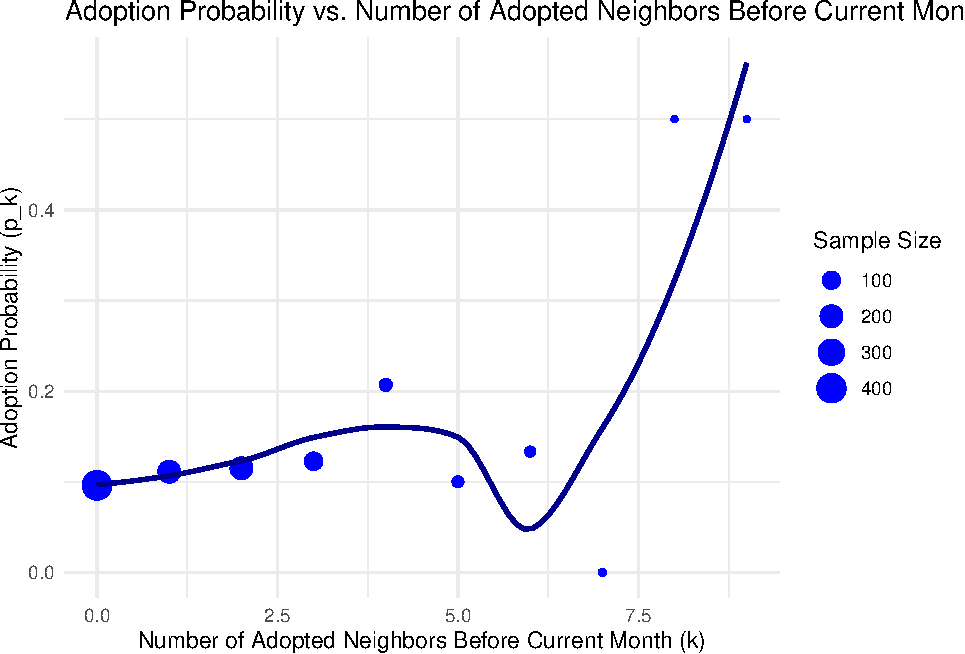
\includegraphics{Homework-04_files/figure-latex/unnamed-chunk-3-1.pdf}
\#\#\#\# c.~

Create a vector of estimated \(q_k\) probabilities, using the data frame
from (2). Plot the probabilities against the number of
prior-or-contemporary-adoptee contacts \(k\).

用以下代码解决

\begin{Shaded}
\begin{Highlighting}[]
\CommentTok{\# 计算 q\_k}
\NormalTok{q\_data }\OtherTok{\textless{}{-}}\NormalTok{ doctor\_months }\SpecialCharTok{\%\textgreater{}\%}
\FunctionTok{filter}\NormalTok{(already\_adopted }\SpecialCharTok{==} \DecValTok{0}\NormalTok{) }\SpecialCharTok{\%\textgreater{}\%} \CommentTok{\# 只考虑尚未采用的医生}
\FunctionTok{group\_by}\NormalTok{(n\_contacts\_adopted\_by\_now) }\SpecialCharTok{\%\textgreater{}\%}
\FunctionTok{summarise}\NormalTok{(}
\AttributeTok{q\_k =} \FunctionTok{mean}\NormalTok{(adopted\_this\_month),}
\AttributeTok{count =} \FunctionTok{n}\NormalTok{()}
\NormalTok{) }\SpecialCharTok{\%\textgreater{}\%}
  \FunctionTok{rename}\NormalTok{(}\AttributeTok{k =}\NormalTok{ n\_contacts\_adopted\_by\_now)}
\CommentTok{\# Plot}
\FunctionTok{ggplot}\NormalTok{(q\_data, }\FunctionTok{aes}\NormalTok{(}\AttributeTok{x =}\NormalTok{ k, }\AttributeTok{y =}\NormalTok{ q\_k)) }\SpecialCharTok{+}
\FunctionTok{geom\_point}\NormalTok{(}\FunctionTok{aes}\NormalTok{(}\AttributeTok{size =}\NormalTok{ count), }\AttributeTok{color =} \StringTok{"red"}\NormalTok{) }\SpecialCharTok{+}
\FunctionTok{geom\_smooth}\NormalTok{(}\AttributeTok{method =} \StringTok{"loess"}\NormalTok{, }\AttributeTok{se =} \ConstantTok{FALSE}\NormalTok{, }\AttributeTok{color =} \StringTok{"darkred"}\NormalTok{) }\SpecialCharTok{+}
\FunctionTok{labs}\NormalTok{(}
\AttributeTok{title =} \StringTok{"Adoption Probability vs. Number of Adopted Neighbors Up to Current Month (q\_k)"}\NormalTok{,}
\AttributeTok{x =} \StringTok{"Number of Adopted Neighbors Up to Current Month (k)"}\NormalTok{,}
\AttributeTok{y =} \StringTok{"Adoption Probability (q\_k)"}
\NormalTok{) }\SpecialCharTok{+}
\FunctionTok{scale\_size\_continuous}\NormalTok{(}\AttributeTok{name =} \StringTok{"Sample Size"}\NormalTok{) }\SpecialCharTok{+}
\FunctionTok{theme\_minimal}\NormalTok{()}
\end{Highlighting}
\end{Shaded}

\begin{verbatim}
## `geom_smooth()` using formula = 'y ~ x'
\end{verbatim}

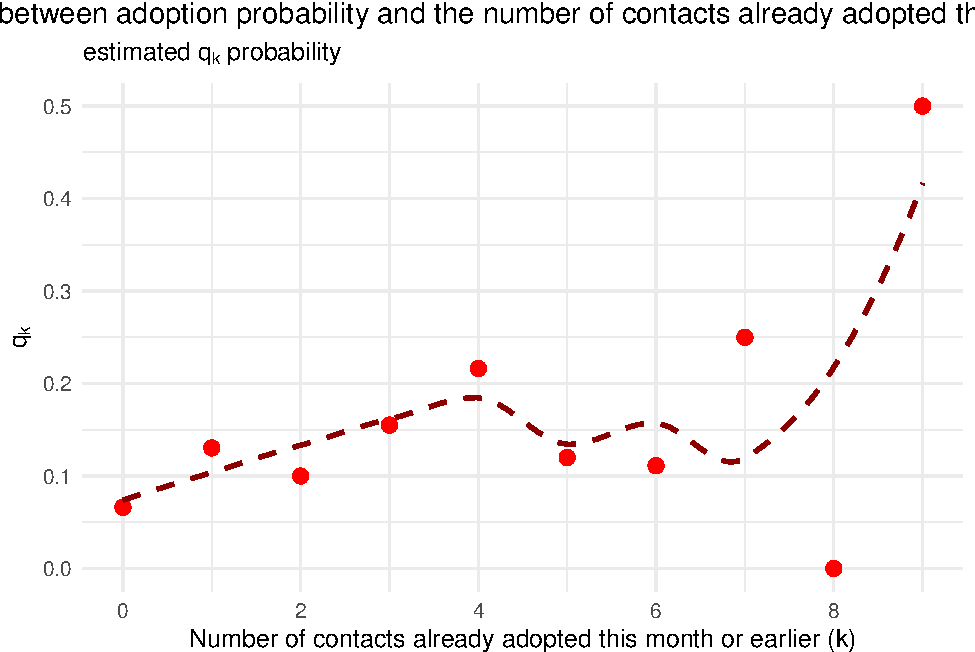
\includegraphics{Homework-04_files/figure-latex/unnamed-chunk-4-1.pdf}

\subsubsection{4.}\label{section-3}

Because it only conditions on information from the previous month,
\(p_k\) is a little easier to interpret than \(q_k\). It is the
probability per month that a doctor adopts tetracycline, if they have
exactly \(k\) contacts who had already adopted tetracycline.

\paragraph{a.}\label{a.-1}

Suppose \(p_k = a + bk\). This would mean that each friend who adopts
the new drug increases the probability of adoption by an equal amount.
Estimate this model by least squares, using the values you constructed
in (3b). Report the parameter estimates.

用以下代码解决:

\begin{Shaded}
\begin{Highlighting}[]
\CommentTok{\# 使用加权最小二乘法估计线性模型(权重为样本量)}
\NormalTok{linear\_model }\OtherTok{\textless{}{-}} \FunctionTok{lm}\NormalTok{(p\_k }\SpecialCharTok{\textasciitilde{}}\NormalTok{ k, }\AttributeTok{data =}\NormalTok{ p\_data, }\AttributeTok{weights =}\NormalTok{ count)}
\CommentTok{\# 获取参数估计}
\NormalTok{linear\_coef }\OtherTok{\textless{}{-}} \FunctionTok{coef}\NormalTok{(linear\_model)}
\FunctionTok{cat}\NormalTok{(}\StringTok{" 线性模型估计结果:}\SpecialCharTok{\textbackslash{}n}\StringTok{"}\NormalTok{)}
\end{Highlighting}
\end{Shaded}

\begin{verbatim}
##  线性模型估计结果:
\end{verbatim}

\begin{Shaded}
\begin{Highlighting}[]
\FunctionTok{cat}\NormalTok{(}\FunctionTok{sprintf}\NormalTok{(}\StringTok{" 截距 a = \%.4f}\SpecialCharTok{\textbackslash{}n}\StringTok{斜率 b = \%.4f"}\NormalTok{, linear\_coef[}\DecValTok{1}\NormalTok{], linear\_coef[}\DecValTok{2}\NormalTok{]))}
\end{Highlighting}
\end{Shaded}

\begin{verbatim}
##  截距 a = 0.0947
## 斜率 b = 0.0126
\end{verbatim}

\paragraph{b.}\label{b.-1}

Suppose \(p_k = e^{a+bk}/(1+e^{a+bk})\). Explain, in words, what this
model would imply about the impact of adding one more adoptee friend on
a given doctor's probability of adoption. (You can suppose that
\(b > 0\), if that makes it easier.) Estimate the model by least
squares, using the values you constructed in (3b).

用以下代码解决:

\begin{Shaded}
\begin{Highlighting}[]
\CommentTok{\# 使用加权非线性最小二乘法估计 logistic 模型}
\NormalTok{logistic\_model }\OtherTok{\textless{}{-}} \FunctionTok{nls}\NormalTok{(}
\NormalTok{p\_k }\SpecialCharTok{\textasciitilde{}} \FunctionTok{exp}\NormalTok{(a }\SpecialCharTok{+}\NormalTok{ b}\SpecialCharTok{*}\NormalTok{k)}\SpecialCharTok{/}\NormalTok{(}\DecValTok{1} \SpecialCharTok{+} \FunctionTok{exp}\NormalTok{(a }\SpecialCharTok{+}\NormalTok{ b}\SpecialCharTok{*}\NormalTok{k)),}
\AttributeTok{data =}\NormalTok{ p\_data,}
\AttributeTok{weights =}\NormalTok{ count,}
\AttributeTok{start =} \FunctionTok{list}\NormalTok{(}\AttributeTok{a =} \SpecialCharTok{{-}}\DecValTok{4}\NormalTok{, }\AttributeTok{b =} \FloatTok{0.1}\NormalTok{) }\CommentTok{\# 初始值}
\NormalTok{)}
\CommentTok{\# 获取参数估计}
\NormalTok{logistic\_coef }\OtherTok{\textless{}{-}} \FunctionTok{coef}\NormalTok{(logistic\_model)}
\FunctionTok{cat}\NormalTok{(}\StringTok{"}\SpecialCharTok{\textbackslash{}n}\StringTok{Logistic 模型估计结果:}\SpecialCharTok{\textbackslash{}n}\StringTok{"}\NormalTok{)}
\end{Highlighting}
\end{Shaded}

\begin{verbatim}
## 
## Logistic 模型估计结果:
\end{verbatim}

\begin{Shaded}
\begin{Highlighting}[]
\FunctionTok{cat}\NormalTok{(}\FunctionTok{sprintf}\NormalTok{(}\StringTok{" 参数 a = \%.4f}\SpecialCharTok{\textbackslash{}n}\StringTok{参数 b = \%.4f"}\NormalTok{, logistic\_coef[}\DecValTok{1}\NormalTok{], logistic\_coef[}\DecValTok{2}\NormalTok{]))}
\end{Highlighting}
\end{Shaded}

\begin{verbatim}
##  参数 a = -2.2548
## 参数 b = 0.1229
\end{verbatim}

\paragraph{c.~}\label{c.}

Plot the values from (3b) along with the estimated curves from (4a) and
(4b). (You should have one plot, with \(k\) on the horizontal axis, and
probabilities on the vertical axis .) Which model do you prefer, and
why?

用以下代码解决:

\begin{Shaded}
\begin{Highlighting}[]
\CommentTok{\# 生成预测数据}
\NormalTok{k\_range }\OtherTok{\textless{}{-}} \DecValTok{0}\SpecialCharTok{:}\DecValTok{20}
\NormalTok{linear\_pred }\OtherTok{\textless{}{-}}\NormalTok{ linear\_coef[}\DecValTok{1}\NormalTok{] }\SpecialCharTok{+}\NormalTok{ linear\_coef[}\DecValTok{2}\NormalTok{]}\SpecialCharTok{*}\NormalTok{k\_range}
\NormalTok{logistic\_pred }\OtherTok{\textless{}{-}} \FunctionTok{exp}\NormalTok{(logistic\_coef[}\DecValTok{1}\NormalTok{] }\SpecialCharTok{+}\NormalTok{ logistic\_coef[}\DecValTok{2}\NormalTok{]}\SpecialCharTok{*}\NormalTok{k\_range)}\SpecialCharTok{/}
\NormalTok{(}\DecValTok{1} \SpecialCharTok{+} \FunctionTok{exp}\NormalTok{(logistic\_coef[}\DecValTok{1}\NormalTok{] }\SpecialCharTok{+}\NormalTok{ logistic\_coef[}\DecValTok{2}\NormalTok{]}\SpecialCharTok{*}\NormalTok{k\_range))}
\CommentTok{\# 创建比较数据框}
\NormalTok{comparison\_df }\OtherTok{\textless{}{-}} \FunctionTok{data.frame}\NormalTok{(}
\AttributeTok{k =} \FunctionTok{rep}\NormalTok{(k\_range, }\DecValTok{3}\NormalTok{),}
\AttributeTok{Probability =} \FunctionTok{c}\NormalTok{(p\_data}\SpecialCharTok{$}\NormalTok{p\_k[}\FunctionTok{match}\NormalTok{(k\_range, p\_data}\SpecialCharTok{$}\NormalTok{k)],}
\NormalTok{linear\_pred,}
\NormalTok{logistic\_pred),}
\AttributeTok{Type =} \FunctionTok{rep}\NormalTok{(}\FunctionTok{c}\NormalTok{(}\StringTok{"Observed"}\NormalTok{, }\StringTok{"Linear"}\NormalTok{, }\StringTok{"Logistic"}\NormalTok{), }\AttributeTok{each =} \FunctionTok{length}\NormalTok{(k\_range))}
\NormalTok{)}
\CommentTok{\# 绘图}
\FunctionTok{ggplot}\NormalTok{(comparison\_df, }\FunctionTok{aes}\NormalTok{(}\AttributeTok{x =}\NormalTok{ k, }\AttributeTok{y =}\NormalTok{ Probability, }\AttributeTok{color =}\NormalTok{ Type)) }\SpecialCharTok{+}
\FunctionTok{geom\_point}\NormalTok{(}\AttributeTok{data =} \FunctionTok{subset}\NormalTok{(comparison\_df, Type }\SpecialCharTok{==} \StringTok{"Observed"}\NormalTok{),}
\FunctionTok{aes}\NormalTok{(}\AttributeTok{size =}\NormalTok{ p\_data}\SpecialCharTok{$}\NormalTok{count[}\FunctionTok{match}\NormalTok{(k\_range, p\_data}\SpecialCharTok{$}\NormalTok{k)])) }\SpecialCharTok{+}
\FunctionTok{geom\_line}\NormalTok{(}\AttributeTok{data =} \FunctionTok{subset}\NormalTok{(comparison\_df, Type }\SpecialCharTok{!=} \StringTok{"Observed"}\NormalTok{),}
\AttributeTok{linewidth =} \FloatTok{1.2}\NormalTok{) }\SpecialCharTok{+}
\FunctionTok{scale\_color\_manual}\NormalTok{(}\AttributeTok{values =} \FunctionTok{c}\NormalTok{(}\StringTok{"Observed"} \OtherTok{=} \StringTok{"black"}\NormalTok{,}
\StringTok{"Linear"} \OtherTok{=} \StringTok{"blue"}\NormalTok{,}
\StringTok{"Logistic"} \OtherTok{=} \StringTok{"red"}\NormalTok{)) }\SpecialCharTok{+}
\FunctionTok{labs}\NormalTok{(}\AttributeTok{title =} \StringTok{"Comparison of Adoption Probability Models"}\NormalTok{,}
\AttributeTok{x =} \StringTok{"Number of Prior{-}Adoptee Contacts (k)"}\NormalTok{,}
\AttributeTok{y =} \StringTok{"Adoption Probability (p\_k)"}\NormalTok{,}
\AttributeTok{color =} \StringTok{"Model Type"}\NormalTok{) }\SpecialCharTok{+}
\FunctionTok{scale\_size\_continuous}\NormalTok{(}\AttributeTok{name =} \StringTok{"Sample Size"}\NormalTok{, }\AttributeTok{range =} \FunctionTok{c}\NormalTok{(}\DecValTok{2}\NormalTok{, }\DecValTok{6}\NormalTok{)) }\SpecialCharTok{+}
\FunctionTok{theme\_minimal}\NormalTok{() }\SpecialCharTok{+}
\FunctionTok{theme}\NormalTok{(}\AttributeTok{legend.position =} \StringTok{"bottom"}\NormalTok{)}
\end{Highlighting}
\end{Shaded}

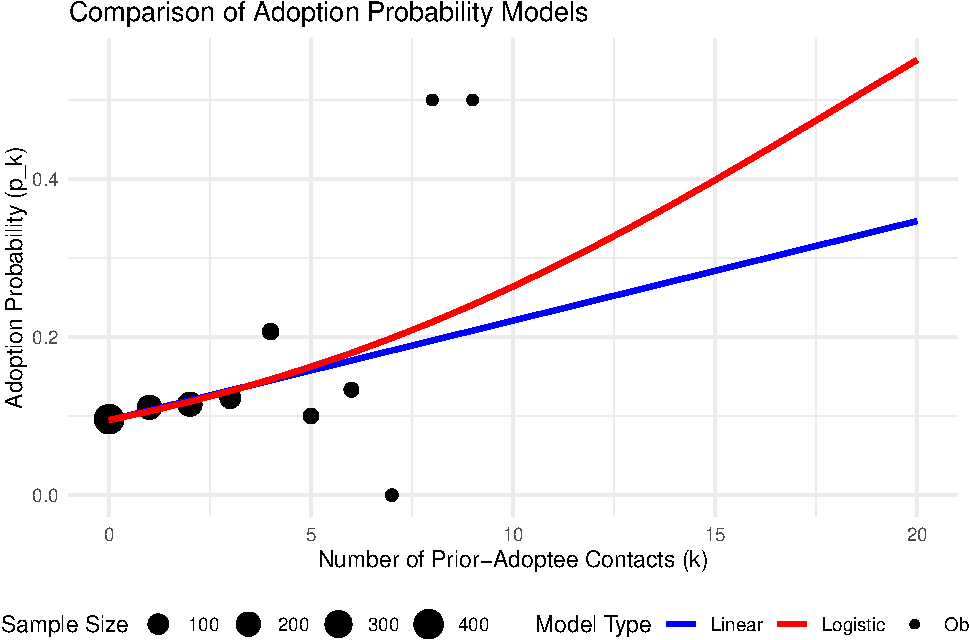
\includegraphics{Homework-04_files/figure-latex/unnamed-chunk-7-1.pdf}

\emph{For quibblers, pedants, and idle hands itching for work to do}:
The \(p_k\) values from problem 3 aren't all equally precise, because
they come from different numbers of observations. Also, if each doctor
with \(k\) adoptee contacts is independently deciding whether or not to
adopt with probability \(p_k\), then the variance in the number of
adoptees will depend on \(p_k\). Say that the actual proportion who
decide to adopt is \(\hat{p}_k\). A little probability (exercise!) shows
that in this situation, \(\mathbb{E}[\hat{p}_k] = p_k\), but that
\(\mathrm{Var}[\hat{p}_k] = p_k(1-p_k)/n_k\), where \(n_k\) is the
number of doctors in that situation. (We estimate probabilities more
precisely when they're really extreme {[}close to 0 or 1{]}, and/or we
have lots of observations.) We can estimate that variance as
\(\hat{V}_k = \hat{p}_k(1-\hat{p}_k)/n_k\). Find the \(\hat{V}_k\), and
then re-do the estimation in (4a) and (4b) where the squared error for
\(p_k\) is divided by \(\hat{V}_k\). How much do the parameter estimates
change? How much do the plotted curves in (4c) change?

用以下代码解决:

\begin{Shaded}
\begin{Highlighting}[]
\CommentTok{\# 基于问题 3b 的 p\_data 计算方差估计}
\NormalTok{p\_data }\OtherTok{\textless{}{-}}\NormalTok{ p\_data }\SpecialCharTok{\%\textgreater{}\%}
\FunctionTok{mutate}\NormalTok{(}
\AttributeTok{V\_k =}\NormalTok{ p\_k }\SpecialCharTok{*}\NormalTok{ (}\DecValTok{1} \SpecialCharTok{{-}}\NormalTok{ p\_k) }\SpecialCharTok{/}\NormalTok{ count, }\CommentTok{\# 方差估计}
\AttributeTok{weight =} \FunctionTok{ifelse}\NormalTok{(V\_k }\SpecialCharTok{\textgreater{}} \DecValTok{0}\NormalTok{, }\DecValTok{1}\SpecialCharTok{/}\NormalTok{V\_k, }\DecValTok{0}\NormalTok{) }\CommentTok{\# 权重(方差的倒数)}
\NormalTok{) }\SpecialCharTok{\%\textgreater{}\%}
\FunctionTok{filter}\NormalTok{(}\SpecialCharTok{!}\FunctionTok{is.na}\NormalTok{(V\_k) }\SpecialCharTok{\&} \FunctionTok{is.finite}\NormalTok{(V\_k)) }\CommentTok{\# 移除无效值}
\CommentTok{\# 加权线性回归}
\NormalTok{weighted\_linear\_model }\OtherTok{\textless{}{-}} \FunctionTok{lm}\NormalTok{(p\_k }\SpecialCharTok{\textasciitilde{}}\NormalTok{ k, }\AttributeTok{data =}\NormalTok{ p\_data, }\AttributeTok{weights =}\NormalTok{ weight)}
\NormalTok{weighted\_linear\_coef }\OtherTok{\textless{}{-}} \FunctionTok{coef}\NormalTok{(weighted\_linear\_model)}
\CommentTok{\# 加权非线性回归}
\NormalTok{weighted\_logistic\_model }\OtherTok{\textless{}{-}} \FunctionTok{nls}\NormalTok{(}
\NormalTok{p\_k }\SpecialCharTok{\textasciitilde{}} \FunctionTok{exp}\NormalTok{(a }\SpecialCharTok{+}\NormalTok{ b}\SpecialCharTok{*}\NormalTok{k)}\SpecialCharTok{/}\NormalTok{(}\DecValTok{1} \SpecialCharTok{+} \FunctionTok{exp}\NormalTok{(a }\SpecialCharTok{+}\NormalTok{ b}\SpecialCharTok{*}\NormalTok{k)),}
\AttributeTok{data =}\NormalTok{ p\_data,}
\AttributeTok{weights =}\NormalTok{ weight,}
\AttributeTok{start =} \FunctionTok{list}\NormalTok{(}\AttributeTok{a =} \SpecialCharTok{{-}}\DecValTok{4}\NormalTok{, }\AttributeTok{b =} \FloatTok{0.1}\NormalTok{)}
\NormalTok{)}
\NormalTok{weighted\_logistic\_coef }\OtherTok{\textless{}{-}} \FunctionTok{coef}\NormalTok{(weighted\_logistic\_model)}
\end{Highlighting}
\end{Shaded}

\subsubsection{参数比较}\label{ux53c2ux6570ux6bd4ux8f83}

\begin{Shaded}
\begin{Highlighting}[]
\CommentTok{\# 创建参数比较表格}
\NormalTok{param\_comparison }\OtherTok{\textless{}{-}} \FunctionTok{data.frame}\NormalTok{(}
\AttributeTok{Model =} \FunctionTok{c}\NormalTok{(}\StringTok{"Linear"}\NormalTok{, }\StringTok{"Linear (Weighted)"}\NormalTok{, }\StringTok{"Logistic"}\NormalTok{, }\StringTok{"Logistic (Weighted)"}\NormalTok{),}
\AttributeTok{a =} \FunctionTok{c}\NormalTok{(linear\_coef[}\DecValTok{1}\NormalTok{], weighted\_linear\_coef[}\DecValTok{1}\NormalTok{],}
\NormalTok{logistic\_coef[}\DecValTok{1}\NormalTok{], weighted\_logistic\_coef[}\DecValTok{1}\NormalTok{]),}
\AttributeTok{b =} \FunctionTok{c}\NormalTok{(linear\_coef[}\DecValTok{2}\NormalTok{], weighted\_linear\_coef[}\DecValTok{2}\NormalTok{],}
\NormalTok{logistic\_coef[}\DecValTok{2}\NormalTok{], weighted\_logistic\_coef[}\DecValTok{2}\NormalTok{])}
\NormalTok{)}
\CommentTok{\# 计算变化百分比}
\NormalTok{param\_comparison }\OtherTok{\textless{}{-}}\NormalTok{ param\_comparison }\SpecialCharTok{\%\textgreater{}\%}
\FunctionTok{mutate}\NormalTok{(}
\AttributeTok{a\_change =} \FunctionTok{c}\NormalTok{(}\DecValTok{0}\NormalTok{, }\DecValTok{100}\SpecialCharTok{*}\NormalTok{(a[}\DecValTok{2}\NormalTok{]}\SpecialCharTok{{-}}\NormalTok{a[}\DecValTok{1}\NormalTok{])}\SpecialCharTok{/}\NormalTok{a[}\DecValTok{1}\NormalTok{], }\DecValTok{0}\NormalTok{, }\DecValTok{100}\SpecialCharTok{*}\NormalTok{(a[}\DecValTok{4}\NormalTok{]}\SpecialCharTok{{-}}\NormalTok{a[}\DecValTok{3}\NormalTok{])}\SpecialCharTok{/}\NormalTok{a[}\DecValTok{3}\NormalTok{]),}
\AttributeTok{b\_change =} \FunctionTok{c}\NormalTok{(}\DecValTok{0}\NormalTok{, }\DecValTok{100}\SpecialCharTok{*}\NormalTok{(b[}\DecValTok{2}\NormalTok{]}\SpecialCharTok{{-}}\NormalTok{b[}\DecValTok{1}\NormalTok{])}\SpecialCharTok{/}\NormalTok{b[}\DecValTok{1}\NormalTok{], }\DecValTok{0}\NormalTok{, }\DecValTok{100}\SpecialCharTok{*}\NormalTok{(b[}\DecValTok{4}\NormalTok{]}\SpecialCharTok{{-}}\NormalTok{b[}\DecValTok{3}\NormalTok{])}\SpecialCharTok{/}\NormalTok{b[}\DecValTok{3}\NormalTok{])}
\NormalTok{)}
\FunctionTok{print}\NormalTok{(param\_comparison)}
\end{Highlighting}
\end{Shaded}

\begin{verbatim}
##                 Model           a          b  a_change  b_change
## 1              Linear  0.09470668 0.01260200  0.000000   0.00000
## 2   Linear (Weighted)  0.09637512 0.01050772  1.761692 -16.61857
## 3            Logistic -2.25484997 0.12288660  0.000000   0.00000
## 4 Logistic (Weighted) -2.23476722 0.10372101 -0.890647 -15.59616
\end{verbatim}

\subsubsection{曲线比较}\label{ux66f2ux7ebfux6bd4ux8f83}

\begin{Shaded}
\begin{Highlighting}[]
\CommentTok{\# 生成预测数据}
\NormalTok{k\_range }\OtherTok{\textless{}{-}} \DecValTok{0}\SpecialCharTok{:}\DecValTok{20}
\NormalTok{orig\_linear }\OtherTok{\textless{}{-}}\NormalTok{ linear\_coef[}\DecValTok{1}\NormalTok{] }\SpecialCharTok{+}\NormalTok{ linear\_coef[}\DecValTok{2}\NormalTok{]}\SpecialCharTok{*}\NormalTok{k\_range}
\NormalTok{weighted\_linear }\OtherTok{\textless{}{-}}\NormalTok{ weighted\_linear\_coef[}\DecValTok{1}\NormalTok{] }\SpecialCharTok{+}\NormalTok{ weighted\_linear\_coef[}\DecValTok{2}\NormalTok{]}\SpecialCharTok{*}\NormalTok{k\_range}
\NormalTok{orig\_logistic }\OtherTok{\textless{}{-}} \FunctionTok{exp}\NormalTok{(logistic\_coef[}\DecValTok{1}\NormalTok{] }\SpecialCharTok{+}\NormalTok{ logistic\_coef[}\DecValTok{2}\NormalTok{]}\SpecialCharTok{*}\NormalTok{k\_range)}\SpecialCharTok{/}
\NormalTok{(}\DecValTok{1} \SpecialCharTok{+} \FunctionTok{exp}\NormalTok{(logistic\_coef[}\DecValTok{1}\NormalTok{] }\SpecialCharTok{+}\NormalTok{ logistic\_coef[}\DecValTok{2}\NormalTok{]}\SpecialCharTok{*}\NormalTok{k\_range))}
\NormalTok{weighted\_logistic }\OtherTok{\textless{}{-}} \FunctionTok{exp}\NormalTok{(weighted\_logistic\_coef[}\DecValTok{1}\NormalTok{] }\SpecialCharTok{+}\NormalTok{ weighted\_logistic\_coef[}\DecValTok{2}\NormalTok{]}\SpecialCharTok{*}\NormalTok{k\_range)}\SpecialCharTok{/}
\NormalTok{(}\DecValTok{1} \SpecialCharTok{+} \FunctionTok{exp}\NormalTok{(weighted\_logistic\_coef[}\DecValTok{1}\NormalTok{] }\SpecialCharTok{+}\NormalTok{ weighted\_logistic\_coef[}\DecValTok{2}\NormalTok{]}\SpecialCharTok{*}\NormalTok{k\_range))}
\CommentTok{\# 创建比较数据框}
\NormalTok{curve\_comparison }\OtherTok{\textless{}{-}} \FunctionTok{data.frame}\NormalTok{(}
\AttributeTok{k =} \FunctionTok{rep}\NormalTok{(k\_range, }\DecValTok{4}\NormalTok{),}
\AttributeTok{Probability =} \FunctionTok{c}\NormalTok{(orig\_linear, weighted\_linear, orig\_logistic, weighted\_logistic),}
\AttributeTok{Model =} \FunctionTok{rep}\NormalTok{(}\FunctionTok{c}\NormalTok{(}\StringTok{"Linear"}\NormalTok{, }\StringTok{"Linear (Weighted)"}\NormalTok{, }\StringTok{"Logistic"}\NormalTok{, }\StringTok{"Logistic (Weighted)"}\NormalTok{),}
\AttributeTok{each =} \FunctionTok{length}\NormalTok{(k\_range))}
\NormalTok{)}
\CommentTok{\# 绘图}
\FunctionTok{ggplot}\NormalTok{(curve\_comparison, }\FunctionTok{aes}\NormalTok{(}\AttributeTok{x =}\NormalTok{ k, }\AttributeTok{y =}\NormalTok{ Probability, }\AttributeTok{color =}\NormalTok{ Model, }\AttributeTok{linetype =}\NormalTok{ Model)) }\SpecialCharTok{+}
\FunctionTok{geom\_line}\NormalTok{(}\AttributeTok{linewidth =} \FloatTok{1.2}\NormalTok{) }\SpecialCharTok{+}
\FunctionTok{geom\_point}\NormalTok{(}\AttributeTok{data =}\NormalTok{ p\_data, }\FunctionTok{aes}\NormalTok{(}\AttributeTok{x =}\NormalTok{ k, }\AttributeTok{y =}\NormalTok{ p\_k, }\AttributeTok{size =}\NormalTok{ count),}
\AttributeTok{color =} \StringTok{"black"}\NormalTok{, }\AttributeTok{inherit.aes =} \ConstantTok{FALSE}\NormalTok{) }\SpecialCharTok{+}
\FunctionTok{scale\_color\_manual}\NormalTok{(}\AttributeTok{values =} \FunctionTok{c}\NormalTok{(}\StringTok{"Linear"} \OtherTok{=} \StringTok{"blue"}\NormalTok{, }\StringTok{"Linear (Weighted)"} \OtherTok{=} \StringTok{"dodgerblue"}\NormalTok{,}
\StringTok{"Logistic"} \OtherTok{=} \StringTok{"red"}\NormalTok{, }\StringTok{"Logistic (Weighted)"} \OtherTok{=} \StringTok{"salmon"}\NormalTok{)) }\SpecialCharTok{+}
\FunctionTok{scale\_linetype\_manual}\NormalTok{(}\AttributeTok{values =} \FunctionTok{c}\NormalTok{(}\StringTok{"Linear"} \OtherTok{=} \StringTok{"solid"}\NormalTok{, }\StringTok{"Linear (Weighted)"} \OtherTok{=} \StringTok{"dashed"}\NormalTok{,}
\StringTok{"Logistic"} \OtherTok{=} \StringTok{"solid"}\NormalTok{, }\StringTok{"Logistic (Weighted)"} \OtherTok{=} \StringTok{"dashed"}\NormalTok{)) }\SpecialCharTok{+}
\FunctionTok{labs}\NormalTok{(}\AttributeTok{title =} \StringTok{"Weighted vs Unweighted Model Comparison"}\NormalTok{,}
\AttributeTok{subtitle =} \StringTok{"Points show observed probabilities (size = sample size)"}\NormalTok{,}
\AttributeTok{x =} \StringTok{"Number of Prior{-}Adoptee Contacts (k)"}\NormalTok{,}
\AttributeTok{y =} \StringTok{"Adoption Probability (p\_k)"}\NormalTok{) }\SpecialCharTok{+}
\FunctionTok{scale\_size\_continuous}\NormalTok{(}\AttributeTok{name =} \StringTok{"Sample Size"}\NormalTok{, }\AttributeTok{range =} \FunctionTok{c}\NormalTok{(}\DecValTok{2}\NormalTok{, }\DecValTok{6}\NormalTok{)) }\SpecialCharTok{+}
\FunctionTok{theme\_minimal}\NormalTok{() }\SpecialCharTok{+}
\FunctionTok{theme}\NormalTok{(}\AttributeTok{legend.position =} \StringTok{"bottom"}\NormalTok{)}
\end{Highlighting}
\end{Shaded}

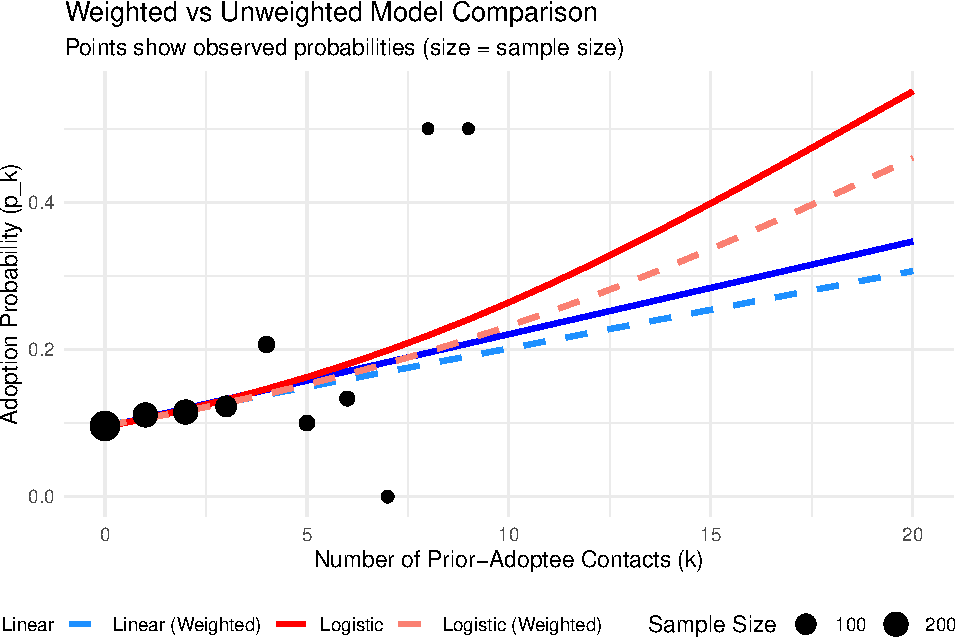
\includegraphics{Homework-04_files/figure-latex/unnamed-chunk-10-1.pdf}

通过比较可以发现,Logistic
模型参数变化较小,更稳健,受加权影响较小;加权估计降低了对样本
量小、高方差数据点的敏感性,更准确地反映了高精度估计(大样本量点)的影响。因此,加权
Logistic 模 型平衡了拟合优度和稳定性。

\end{document}
